\documentclass[main.tex]{subfiles}

\begin{document}

\vspace{1em}

\section*{2.1 The Sky Above}

\textbf{Learning Objectives}
\vspace{-1em}

\begin{itemize}
\setlength\itemsep{0.1ex}
    \item Define the main features of the celestial sphere
    \item Explain the system astronomers use to describe the sky
    \item Describe how motions of the stars appear to us on Earth
    \item Describe how motions of the Sun, Moon, and planets appear to us on Earth
    \item Understand the modern meaning of the term constellation
\end{itemize}

\gls{cardinal directions}: north (N), south (S), east (E), west (W)

\gls{geocentric}: centered on Earth

\subsection*{The Celestial Sphere}

\gls{celestial sphere}: spherical (ball-like) shape of sky; dome where stars are fixed


\gls{zenith}: point on celestial sphere directly above you; look up!

\gls{horizon}: circle around you where dome of sky meets Earth

\begin{figure}[h!]
    \centering
\begin{tikzpicture}
\def\R{2.5} % sphere radius
\def\angEl{10} % elevation angle
\def\angBeta{25} % latitude of point P and Q


\pgfmathsetmacro\H{\R*cos(\angEl)} % distance to north pole
\node at (-0.2,0.7) {\small \textbf{E}};
\shade[ball color=white,opacity=0.5] (0,0) circle (\R);
\coordinate[mark coordinate] (O) at (0,0);

\begin{scope}[rotate=30]
    \DrawLatitudeCircleBack[\R]{0}
\end{scope}

\FillLatitudeCircle[\R]{0}
\DrawLatitudeCircle[\R]{0}

\draw[->] (0,0.15*\R) -- (0,1.01*\R) node[above] {Zenith};

\begin{scope}[rotate=30]
    \draw[thick] (0,\R) -- (0,\R*1.25) node[left=1pt,align=left] {North \\celestial\\ pole} (0,-\R) -- (0,-\R*1.25) node[right=1pt,align=left] {South \\celestial\\ pole};
    \draw[dashed,very thin] (0,\R) -- (0,0.2) (0,-0.22*\R) -- (0,-\R);
    \DrawLatitudeCircleFront[\R]{0}
\end{scope}

\draw (-\R*0.7,-\R*0.52) --++ (-\R*0.2,-\R*0.3) node[below left,align=left] {Celestial\\ equator};
\node[left] at (-\R,0) {\textbf{N}};
\node[right] at (\R,0) {\textbf{S}};
\draw (2,0.25) -- ++(1,0.7) node[right] {Horizon};

\node at (0,0.1) {\Strichmaxerl[1.8]};
\node at (1.3*\R,0.9*\R) {\large \textbf{Celestial Sphere}};
\node at (0.1,-\R*0.3) {\textbf{W}};
\end{tikzpicture}
\caption*{\textbf{Figure 2.3 Circles on the Celestial Sphere.}}
\end{figure}


\subsection*{Celestial Poles and Celestial Equator}

\gls{celestial poles}: point about which celestial sphere rotates

North celestial pole (NCP), south celestial pole (SCP)

\hgraydashline

\gls{constellation}: star patterns on celestial sphere representing ancient stories of people, animals, things

Total 88 constellations across celestial sphere

\framebox{\textbf{Link}} ``Orion'' at \texttt{theoi.com} (\href{https://www.theoi.com/Gigante/GiganteOrion.html}{click here})

\framebox{\textbf{Link}} \textit{YouTube}: ``Zeitgeist: The Movie'' by \texttt{YouTube Movies \& Shows} (\href{https://youtu.be/xM6LXDQXMUw?t=900}{click here}). Good intro to mythology of ``The Three Kings,'' which are also Orion's belt.

\gls{celestial equator}: circle that divides celestial sphere in half

Celestial equator passes near Orion's belt

Location of celestial equator on sky changes depending on your geographical location on Earth

At Ecuador (terrestrial equator, South America), celestial equator passes through zenith

\hgraydashline

\subsection*{Rising and Setting of the Sun}

\framebox{\textbf{Link}} \textit{YouTube}: ``Seasons'' by \texttt{Earth Rocks!} (\href{https://youtu.be/tX3Y5bzNDiU}{click here}). Watch first 2 minutes.

{\color{lightgray} Emphasize that we're still in geocentric view, not yet heliocentric. We need a geocentric model of Sun's yearly path around celestial sphere.}

\gls{year}: 365 days; time it takes Earth to go around Sun once

%Teacher note: Open Stellarium. Place Sun at noonish. Show constellation lines, labels, and art. Then remove atmosphere. Advance the days by 1 day (hold up arrow). Show how Sun advances through 13 zodiacal constellations across the year. Then show ecliptic, the name of this path.
\gls{ecliptic}: Sun's path on the celestial sphere throughout 1 year

\begin{figure}[h!]
\centering
\begin{tikzpicture}

\def\R{3} % sphere radius
\def\angEl{23} % elevation angle
\def\angTilt{30} %tilt angle increased from 23.5 for emphasis

\draw (0,0) -- (0,\R*1.25);

\draw[very thick,fill=yellow] (0.3,1.15) circle (3pt) node[above right] {\textbf{September}};

\begin{scope}[rotate=-\angTilt]
    \draw (0,1.25*\R) -- (0,0);
\end{scope}
\shade[ball color=white, opacity=0.5] (0,0) circle (\R);
\coordinate[mark coordinate] (O) at (0,0);

\begin{scope}[rotate=-\angTilt]
    \DrawLatitudeCircleBack[\R]{0}
\end{scope}

\begin{scope}[rotate=-\angTilt]
        \DrawLatitudeCircleFront[\R]{0}
        \draw[blue,thick]  (0,0) -- (0,1) (0,0) -- (0,-1); %(0,\R*1.25) -- (0,\R)
        \draw[very thick,blue,fill=white] (0,0) circle (19pt) node {\rotatebox{-\angTilt}{\textbf{Earth}}};
        \node at (0.25,0.9) {\textbf{N}};
        \node at (-0.2,-0.9) {\textbf{S}};
\end{scope}

\DrawLatitudeCircle[\R]{0}
\draw (-2,-0.9) --++ (-1.3,-0.6) node[below] {Ecliptic};

\draw[very thick,fill=yellow] (-\R,0) circle (4pt) node[left=7pt] {\textbf{December}};
\draw[very thick,fill=yellow] (\R,0) circle (4pt) node[right=6pt] {\textbf{June}};
\draw[very thick,fill=yellow] (-0.3,-1.15) circle (4pt) node[below=8pt] {\textbf{March}};

\draw[very thick,<->] (0,2.2) arc (90:55:1.85);
\node at (0.75,2.5) {\SI{23.5}{\degree}};

\draw (1.7,-1.8) -- ++(1,-0.4) node[right] {Celestial Equator};

\draw[very thick,<->] (1.7,-1) arc (-10:-45:1.4);
\node at (2.1,-1.45) {\small {\SI{23.5}{\degree}}};

\node at (-2.8,2.8) {Celestial Sphere};

\end{tikzpicture}
\caption*{\textbf{Figure 2.7 The Celestial Tilt}.}
\end{figure}


% \begin{figure}[h!]
% \centering

% \begin{tikzpicture}
% \shade[ball color = lightgray,
%     opacity = 0.15
% ] (0,0,0) circle (3cm);
%     \draw[thick,red] (0,0) ellipse (3cm and 1cm);
%     \draw[thick,dashed,blue,rotate around={-35:(0,0)}] (0,0) ellipse (3cm and 1cm);
%     \draw[thick,red,->] (0,0) -- (0,3);
%     \draw[thick,dashed,blue,->,rotate around={-35:(0,0)}] (0,0) -- (0,3);
%     \draw (-2,-0.75) --++ (-0.8,-0.5) node[anchor=east]{Ecliptic};
%     \draw (-2.4,1) --++ (-0.8,+0.5) node[anchor=east]{Celestial equator};
%     \draw[very thick,<->] (0,2) arc (90:55:2);
%     \node at (0.75,2.3) {\SI{23.5}{\degree}};
%     \draw[very thick,<->] (2,-0.75) arc (-10:-45:2);
% \end{tikzpicture}
% \end{figure}

% \gls{apparent magnitude}

\clearpage
\section*{2.2 Ancient Astronomy}

\def\tick{0.3}
\begin{figure}[h!]
    \centering
    \begin{tikzpicture}[x=0.5cm,y=0.5cm]
    \draw (-6,0) -- (20.5,0);
    \draw (-5.35,-\tick) -- ++(0,2*\tick) node[below=22pt] {Pythagoras} node[below=12pt] {530};
    \draw (-3.50,-\tick) -- ++(0,2*\tick) node[above=12pt] {Aristotle} node[above=2pt] {350};
    \draw (0,-\tick) -- ++(0,2*\tick) node[below=12pt] {0} node[below=24pt] {$\leftarrow$ BC \hspace{1ex} AD $\rightarrow$};
    \draw (1.40,-\tick) -- ++(0,2*\tick) node[above] {Ptolemy} node[below=12pt] {140};
    \draw (15.43,-\tick) -- ++(0,2*\tick) node[below=22pt] {Copernicus} node[below=12pt] {1543};
    \draw (16.09,-\tick) -- ++(0,2*\tick) node[above=12pt] {Galileo} node[above=2pt] {1609};
    \draw (20.22,-\tick) -- ++(0,2*\tick) node[above] {Present day} node[below=12pt] {2022};
    \end{tikzpicture}
\end{figure}

\subsection*{Early Greek and Roman Cosmology}

2500 years ago Mediterranean people knew Earth was round

Pythagoras {\color{lightgray} (philosopher/mathematician)} said circles \& spheres are ``perfect forms'' $\Rightarrow$ 

Earth \textit{must} be a sphere

Moon, Sun are spheres $\Rightarrow$ gods must love spheres/circles

Aristotle: tutor of Alexander the Great; major Greek philosopher

Moon blocks sunlight during solar eclipse $\Rightarrow$ Sun is more far away

\begin{figure}[h!]
    \centering
    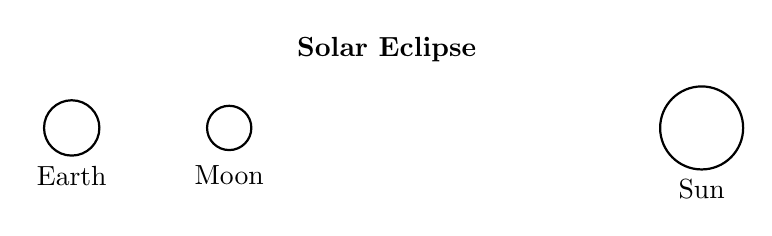
\begin{tikzpicture}
        \draw[thick] (0,0) circle (10pt) node[below=10pt] {Earth};
        \draw[thick] (2,0) circle (8pt) node[below=10pt] {Moon};
        \draw[thick] (8,0) circle (15pt) node[below=15pt] {Sun};
        \node at (4,1) {\textbf{Solar Eclipse}};
    \end{tikzpicture}
\end{figure}

April 8, 2024: next solar eclipse in Texas (Austin)

Aristotle's 2 arguments for round Earth:
\vspace{-1em}

\begin{enumerate}
\setlength\itemsep{0.1ex}
    \item During lunar eclipse, Earth's shadow on Moon is round.
    \item When you travel south, you see new stars on celestial sphere, and North Star gets lower in sky. {\color{lightgray} Use Stellarium to show this. Pick a northern city. Face South, decrease latitude one degree at a time, and observe how celestial sphere reveals more stars.}
\end{enumerate}

{\color{lightgray} Student Lonnie said this was a ``great lesson.''}

\hgraydashline

\subsection*{Ptolemy's Model of the Solar System}

Ptolemy (100--170 AD): last great astronomer of Roman era

Wrote BIG book on astronomy called \textit{Almagest}

Wanted to predict positions of Sun and planets at any date and time

Created geometric model of solar system 

\framebox{\textbf{Link}} AstroSims: Planetary Configurations (\href{https://foothillastrosims.github.io/planetary-config-react/}{click here}). Use this as warm-up.

\framebox{\textbf{Link}} \textit{YouTube}: ``Ptolemy's geocentric universe'' by \texttt{
twistedlot} (\href{https://youtu.be/utH-GHH1FT8}{click here})

Model was predictive tool, not true picture of solar system

Model useful but very complex and required adjustments over time

\hgraydashline

\clearpage
\section*{2.4 The Birth of Modern Astronomy}

% \textbf{Learning Objectives}
% \vspace{-1em}

% \begin{itemize}
% \setlength\itemsep{0.1ex}
%     \item Explain how Copernicus developed the heliocentric model of the solar system
%     \item Explain the Copernican model of planetary motion and describe evidence or arguments in favor of it
%     \item Describe Galileo’s discoveries concerning the study of motion and forces
%     \item Explain how Galileo’s discoveries tilted the balance of evidence in favor of the Copernican model
% \end{itemize}



\subsection*{Copernicus} 

By 1500s old Ptolemaic system needed serious adjustments to work correctly

Nicolaus Copernicus (1473--1543) wanted better theory to calculate planetary positions

In 1543, on death bed, published \textit{On the Revolution of Celestial Orbs}, developed heliocentric model of solar system

\gls{heliocentric}: centered on Sun

Rejected assumption that Earth is center of universe

Believed rotation of celestial sphere is actually rotation of Earth on axis

% \gls{planet}: one of 8 large objects revolving around Sun

Concluded Earth is a planet; all planets circle the Sun

[Draw sketch] Copernicus put Sun at center, planets in order: Mercury, Venus, Earth, Mars, Jupiter, Saturn.

Heliocentrism is a hypothesis: Copernicus didn't prove Earth revolves around Sun

Heliocentric idea was debated for 50+ years

{\color{lightgray} \footnotesize (15 min)}
\vspace{-1ex}

\hgraydashline

\subsection*{Galileo and the Beginning of Modern Science}

Galileo Galilei (1564–1642): mathematician from Pisa, Italy

Galileo adopted Copernican hypothesis of  heliocentric solar system

Roman Catholic Church defended ideas of Aristotle and Ptolemy about the universe

Church needed Earth to be at center of creation

\subsection*{Galileo's Astronomical Observations}

Galileo first to point telescope towards the heavens

Made 4 major astronomical discoveries:
\vspace{-1em}

\begin{enumerate}
\setlength\itemsep{0.1ex}
    \item Stars too faint to be seen with eyes are visible with telescope; Milky Way made of countless stars
    \item Found 4 moons orbitting Jupiter $\Rightarrow$ proof not everything revolves around Earth [insert sketch]
    \item Venus (see problem set 2.4)
    \item Moon (problem set 2.4)
% Found Venus has phases like our Moon $\Rightarrow$ Venus \textit{must} orbit Sun

% On Moon's surface he saw  craters, mountain ranges, valleys, and flat, dark areas    
\end{enumerate}

\framebox{\textbf{Link}} ``The Galileo Project'' by Rice University (\href{http://galileo.rice.edu/}{click here})

After Galileo, cannot deny Copernican (heliocentric) view of universe $\Rightarrow$ 

Earth dethroned from central position in Universe

Galileo charged with house arrest by Church; books forbidden until 1836

Ideas of Copernicus and Galileo began a revolution in our conception of the cosmos.

\clearpage


\printnoidxglossaries

\end{document}